\begin{name}
	% {Phản biện 1: Nguyễn Khánh Trọng \\Phản biện 2: Nguyễn Đức Lợi}
	{Biên soạn \& Phản biện: Nhóm 2}
	{Sở GD \& ĐT Hà Nội (Lần 1)}
\end{name}
\Opensolutionfile{ansbook}[ans/ansb\currfilebase]
\caulc
\Opensolutionfile{ans}[ans/ans\currfilebase-Phan-I]
\begin{ex}%[Dự án 2B30UF-VN-MT-15]%[2-KS-1-SoHaNoi-L1-2026,VM038]%[2D1N3-1]
	\immini[thm]{Cho hàm số $y=f(x)$ có đồ thị như hình vẽ. Tổng của giá trị lớn nhất và giá trị nhỏ nhất của hàm số đã cho trên đoạn $[-2;2]$ bằng
		\choice[2]
			{$-5$}
			{$0$}
			{\True $-6$}
			{$-1$}}
			{
			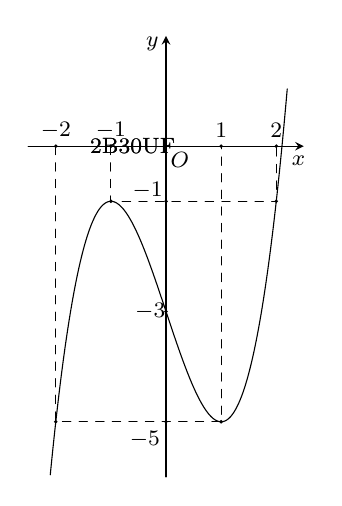
\begin{tikzpicture}[scale=0.7, font=\footnotesize, line join=round, line cap=round, >=stealth]
    %hidden: VM005
				\def \xmin{-2.5}
				\def \xmax{2.5}
				\def \ymin{-6}
				\def \ymax{2}
				\draw[->] (\xmin,0)--(\xmax,0) node[shift=(-110:0.2)] {$x$};
				\draw[->] (0,\ymin)--(0,\ymax) node[shift=(-150:0.2)] {$y$};
				\draw[dashed] (-2,0) -- (-2,-5) -- (1,-5) -- (1,0);
				\draw[dashed] (-1,0) -- (-1,-1) -- (2,-1) -- (2,0) ;
				\draw[smooth, samples=150, domain=-2.1:2.2] plot (\x, {(\x)^3 - 3*(\x) - 3});
				\fill (0,0) node{\href{2B30UF}{\tiny \phantom{2B30UF}}} circle(1pt) node[shift=(-45:0.25)]{$O$}
					(-1,0) circle(1pt) node[shift=(90:0.2)]{$-1$}
					(1,0) circle(1pt) node[shift=(90:0.2)]{$1$}
					(-2,0) circle(1pt) node[shift=(90:0.2)]{$-2$}
					(2,0) circle(1pt) node[shift=(90:0.2)]{$2$}
					(0,-3) circle(1pt) node[shift=(180:0.2)]{$-3$}
					(0,-5) circle(1pt) node[shift=(220:0.35)]{$-5$}
					(0,-1) circle(1pt) node[shift=(150:0.27)]{$-1$}
					(-1,-1) circle(1pt) (2,-1) circle(1pt) 
					(-2,-5) circle(1pt) (1,-5) circle(1pt);
    \node at (0,0){\href{2B30UF}{\tiny \phantom{2B30UF}}};
			\end{tikzpicture}
			}
	\loigiai{
		Quan sát đồ thị hàm số trên đoạn $[-2;2]$, ta thấy
		\begin{itemize}
			\item Giá trị lớn nhất của hàm số là $\max\limits_{[-2;2]} f(x) = -1$ (đạt được tại $x = -1$ và $x = 2$).
			\item Giá trị nhỏ nhất của hàm số là $\min\limits_{[-2;2]} f(x) = -5$ (đạt được tại $x = -2$ và $x = 1$).
		\end{itemize}
		Vậy tổng của giá trị lớn nhất và giá trị nhỏ nhất của hàm số trên đoạn $[-2;2]$ là $-1 + (-5) = -6$.
	}
\end{ex}

\begin{ex}%[Dự án ESAACQ-VN-MT-15]%[2-KS-1-SoHaNoi-L1-2026,VM038]%[2H5N1-2]
	Trong không gian $Oxyz$, cho mặt phẳng $(P)\colon x-2y+2z-1=0$. Một vectơ pháp tuyến của mặt phẳng $(P)$ có tọa độ là
	\choice
		{$(-1;1;2)$}
		{$(1;2;2)$}
		{$(-1;-2;2)$}
		{\True $(1;-2;2)$}
	\loigiai{
		Mặt phẳng $(P)\colon x-2y+2z-1=0$ có một vectơ pháp tuyến là $\overrightarrow{n}=(1;-2;2)$.
	}
\end{ex}

\begin{ex}%[Dự án 3EFEKT-VN-MT-15]%[2-KS-1-SoHaNoi-L1-2026,VM038]%[1D2N3-4]
	Cho cấp số nhân $(u_n)$ có số hạng đầu tiên $u_1=3$ và công bội $q=-2$. Số hạng thứ tư của cấp số nhân đã cho là
	\choice
		{$u_4=48$}
		{$u_4=-48$}
		{$u_4=-4$}
		{\True $u_4=-24$}
	\loigiai{
		Số hạng thứ tư của cấp số nhân là $u_4=u_1 \cdot q^3 = 3\cdot (-2)^3 = 3\cdot (-8) = -24$.
	}
\end{ex}

\begin{ex}%[Dự án 1ZNTFZ-VN-MT-15]%[2-KS-1-SoHaNoi-L1-2026,VM038]%[1D1N4-2]
	Tập xác định của hàm số $y=\tan x$ là
	\choice
		{$\mathbb{R} \setminus \big\{k2\pi \mid k\in \mathbb{Z}\big\}$}
		{\True $\mathbb{R} \setminus \left\{\dfrac{\pi}{2}+k\pi \mid k\in \mathbb{Z}\right\}$}
		{$\mathbb{R} \setminus \left\{\dfrac{\pi}{2}+k2\pi \mid k\in \mathbb{Z}\right\}$}
		{$\mathbb{R} \setminus \big\{k\pi \mid k\in \mathbb{Z}\big\}$}
	\loigiai{
		Hàm số $y=\tan x$ xác định khi $\cos x \ne 0 \Leftrightarrow x \ne \dfrac{\pi}{2}+k\pi$ ($k\in\mathbb{Z}$).\\
		Vậy tập xác định của hàm số là $\mathscr{D} = \mathbb{R} \setminus \left\{\dfrac{\pi}{2}+k\pi \mid k\in \mathbb{Z}\right\}$.
	}
\end{ex}

\begin{ex}%[Dự án 4V2F4J-VN-MT-15]%[2-KS-1-SoHaNoi-L1-2026,VM038]%[1D6H4-3]
	Tập nghiệm của bất phương trình $\log_2 (x-1) \le 3$ là
	\choice
		{$(1;9)$}
		{$(-\infty;9]$}
		{\True $(1;9]$}
		{$[1;9]$}
	\loigiai{
		Điều kiện xác định $x-1 > 0 \Leftrightarrow x > 1$.\\
		Ta có $\log_2 (x-1) \le 3 \Leftrightarrow x-1 \le 2^3\Leftrightarrow x \le 9$.\\
		Kết hợp với điều kiện, ta được $1 < x \le 9$.\\
		Vậy tập nghiệm của bất phương trình là $S=(1;9]$.
	}
\end{ex}

\begin{ex}%[Dự án 3UP5DF-VN-MT-15]%[2-KS-1-SoHaNoi-L1-2026,VM038]%[1D5N1-4]
	Kết quả kiểm tra Toán của $40$ học sinh lớp 12A được cho bởi bảng sau:
	\begin{center}
		\begin{tabular}{|c|c|c|c|c|c|}
			\hline
			\textbf{Khoảng điểm} & $[0;2)$ & $[2;4)$ & $[4;6)$ & $[6;8)$ & $[8;10]$\\
			\hline
			\textbf{Số học sinh} & $0$ & $8$ & $15$ & $10$ & $7$\\
			\hline
		\end{tabular}
	\end{center}
	Mốt của mẫu số liệu ghép nhóm trên thuộc khoảng điểm nào sau đây?
	\choice
		{$[6;8)$}
		{$[8;10]$}
		{\True $[4;6)$}
		{$[2;4)$}
	\loigiai{
		Dựa vào bảng số liệu, ta thấy nhóm $[4;6)$ có tần số lớn nhất (tần số bằng $15$).\\
		Do đó, mốt của mẫu số liệu ghép nhóm trên thuộc khoảng điểm $[4;6)$.
	}
\end{ex}

\begin{ex}%[Dự án XPMRJC-VN-MT-15]%[2-KS-1-SoHaNoi-L1-2026,VM038]%[1H8N7-2]
	\immini[thm]{Cho hình chóp $O.ABC$ có $OA$, $OB$, $OC$ đôi một vuông góc với nhau và $OA=a$, $OB=b$, $OC=c$. Thể tích của khối chóp $O.ABC$ bằng
		\choice[2]
			{$abc$}
			{\True $\dfrac{abc}{6}$}
			{$\dfrac{abc}{3}$}
			{$\dfrac{abc}{2}$}}
			{
			\begin{tikzpicture}[scale=1, font=\footnotesize, line join=round, line cap=round, >=stealth]
    %hidden: VM005
				\coordinate (O) at (0,0);
				\coordinate (B) at (3.5,0);
				\coordinate (C) at (0,3);
				\coordinate (A) at (1.2,-1.5);
				\draw (C) -- (O) -- (A) -- (B) -- (C) -- (A);
				\draw[dashed] (O) -- (B);
				\draw pic[draw, angle radius=2mm] {right angle=C--O--B};
				\draw pic[draw, angle radius=2mm] {right angle=C--O--A};
				\draw[dashed] pic[draw, angle radius=2mm] {right angle=A--O--B};
				\fill (O) circle (1pt) node[left] {$O$};
				\fill (A) circle (1pt) node[below] {$A$};
				\fill (B) circle (1pt) node[right] {$B$};
				\fill (C) circle (1pt) node[above] {$C$};
				\node[left] at ($ (O)!0.5!(C) $) {$c$};
				\node[below left] at ($ (O)!0.5!(A) $) {$a$};
				\node[above] at ($ (O)!0.5!(B) $) {$b$};
    \node at (0,0){\href{XPMRJC}{\tiny \phantom{XPMRJC}}};
			\end{tikzpicture}
			}
	\loigiai{
		Do $OA$, $OB$, $OC$ đôi một vuông góc với nhau nên $OC \perp (OAB)$ và tam giác $OAB$ vuông tại $O$.\\
		Diện tích đáy là $S_{\triangle OAB} = \dfrac{1}{2} OA \cdot OB =\dfrac{1}{2}ab$.\\
		Chiều cao của khối chóp là $h = OC = c$.\\
		Thể tích của khối chóp $O.ABC$ là
		\[V = \dfrac{1}{3} S_{\triangle OAB} \cdot h = \dfrac{1}{3} \cdot \left(\dfrac{1}{2}ab\right) \cdot c = \dfrac{abc}{6}.\]
	}
\end{ex}

\begin{ex}%[Dự án 1EZ324-VN-MT-15]%[2-KS-1-SoHaNoi-L1-2026,VM038]%[2D1N2-2]
	Cho hàm số $y=f(x)$ có đạo hàm trên $\mathbb{R}$ và có bảng xét dấu của $f'(x)$ như sau:
	\begin{center}
		\begin{tikzpicture}
    %hidden: VM005
			\tkzTabInit[nocadre, lgt=1.2, espcl=2.5, deltacl=0.5]
			{$x$ / 0.7, $f'(x)$ / 0.7}
			{$-\infty$, $-3$, $1$, $2$, $+\infty$}
			\tkzTabLine{ , -, 0, +, 0, +, 0, -, }
    \node at (T11){\href{1EZ324}{\tiny \phantom{1EZ324}}};
		\end{tikzpicture}
	\end{center}
	Số điểm cực trị của hàm số $y=f(x)$ là
	\choice
		{$1$}
		{\True $2$}
		{$3$}
		{$0$}
	\loigiai{
		Dựa vào bảng xét dấu đạo hàm, ta thấy $f'(x)$ đổi dấu khi qua $x=-3$ và $x=2$ (không đổi dấu khi qua $x=1$).\\
		Do đó, hàm số đã cho có $2$ điểm cực trị.
	}
\end{ex}

\begin{ex}%[Dự án 392453-VN-MT-15]%[2-KS-1-SoHaNoi-L1-2026,VM038]%[2D4N1-2]
	Họ nguyên hàm của hàm số $f(x)=x^7$ là
	\choice
		{\True $\dfrac{x^8}{8}+C$}
		{$7x^6+C$}
		{$\dfrac{x^7}{7}+C$}
		{$8x^8+C$}
	\loigiai{
		Ta có $\displaystyle\int f(x) \mathrm{\,d}x = \displaystyle\int x^7 \mathrm{\,d}x = \dfrac{x^8}{8} + C$.
	}
\end{ex}

\begin{ex}%[Dự án 3MQVAV-VN-MT-15]%[2-KS-1-SoHaNoi-L1-2026,VM038]%[2D4N3-3]
	Cho hàm số $y=f(x)$ liên tục và không âm trên đoạn $[0;2]$. Thể tích khối tròn xoay sinh ra khi quay quanh trục $Ox$ hình phẳng giới hạn bởi đồ thị hàm số $y=f(x)$, trục hoành và hai đường thẳng $x=0$, $x=2$ là
	\choice
		{\True $\pi \displaystyle\int\limits_0^2 [f(x)]^2 \mathrm{\,d}x$}
		{$\pi \displaystyle\int\limits_0^2 f(x) \mathrm{\,d}x$}
		{$\displaystyle\int\limits_0^2 \big[f(x)\big]^2 \mathrm{\,d}x$}
		{$\displaystyle\int\limits_0^2 f(x) \mathrm{\,d}x$}
	\loigiai{
		Thể tích khối tròn xoay khi quay hình phẳng giới hạn bởi đồ thị hàm số $y=f(x)$ (liên tục và không âm trên $[a;b]$), trục hoành và hai đường thẳng $x=a$, $x=b$ quanh trục $Ox$ là
		\[V = \pi \displaystyle\int\limits_a^b \big[f(x)\big]^2 \mathrm{\,d}x.\]
		Áp dụng với $a=0$, $b=2$, ta được công thức $V = \pi \displaystyle\int\limits_0^2 \big[f(x)\big]^2 \mathrm{\,d}x$.
	}
\end{ex}

\begin{ex}%[Dự án 1MLZYD-VN-MT-15]%[2-KS-1-SoHaNoi-L1-2026,VM038]%[2H2H1-2]
	\immini[thm]{Cho hình hộp $ABCD.A'B'C'D'$ (tham khảo hình vẽ). Khi đó, tổng $\overrightarrow{AB} + \overrightarrow{AD} + \overrightarrow{DD'}$ bằng
		\choice[2]
			{$\overrightarrow{AD'}$}
			{$\overrightarrow{D'A}$}
			{$\overrightarrow{C'A}$}
			{\True $\overrightarrow{AC'}$}}
			{
			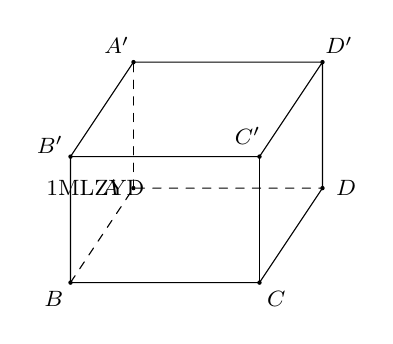
\begin{tikzpicture}[scale=0.8, font=\footnotesize, line join=round, line cap=round, >=stealth]
    %hidden: VM005
				\coordinate (A) at (0,0);
				\coordinate (B) at (-1,-1.5);
				\coordinate (D) at (3,0);
				\coordinate (C) at (2,-1.5);
				\coordinate (A') at (0,2);
				\coordinate (B') at (-1,0.5);
				\coordinate (C') at (2,0.5);
				\coordinate (D') at (3,2);
				\draw (B) -- (C) -- (D) -- (D') -- (C') -- (B') -- cycle;
				\draw (B) -- (B');
				\draw (C) -- (C');
				\draw (D') -- (A') -- (B');
				\draw[dashed] (B) -- (A) -- (D);
				\draw[dashed] (A) -- (A');
				\foreach \i/\j in {A'/135, B'/150, C'/120, D'/45, A/180, B/-135, C/-45, D/0} \fill (\i) node[shift={(\j:3mm)}]{$\i$} circle(1pt);
    \node at (0,0){\href{1MLZYD}{\tiny \phantom{1MLZYD}}};
			\end{tikzpicture}
			}
	\loigiai{
		Vì $ABCD.A'B'C'D'$ là hình hộp nên $\overrightarrow{DD'} = \overrightarrow{CC'}$.\\
		Khi đó
		\[\overrightarrow{AB} + \overrightarrow{AD} + \overrightarrow{DD'} = \overrightarrow{AC} + \overrightarrow{CC'} = \overrightarrow{AC'}.\]
		(Hoặc áp dụng trực tiếp quy tắc hình hộp: $\overrightarrow{AB} + \overrightarrow{AD} + \overrightarrow{AA'} = \overrightarrow{AC'}$, mà $\overrightarrow{AA'} = \overrightarrow{DD'}$).
	}
\end{ex}

\begin{ex}%[Dự án 1D6VDZ-VN-MT-15]%[2-KS-1-SoHaNoi-L1-2026,VM038]%[2H2N2-3]
	Trong không gian $Oxyz$, cho vectơ $\overrightarrow{u} = 3\overrightarrow{i} - 2\overrightarrow{j} + \overrightarrow{k}$. Tọa độ của vectơ $\overrightarrow{u}$ là
	\choice
		{\True $(3;-2;1)$}
		{$(3;1;-2)$}
		{$(1;3;-2)$}
		{$(-2;3;1)$}
	\loigiai{
		Trong hệ trục tọa độ $Oxyz$, vectơ $\overrightarrow{u} = x\overrightarrow{i} + y\overrightarrow{j} + z\overrightarrow{k}$ có tọa độ là $(x;y;z)$.\\
		Suy ra vectơ $\overrightarrow{u} = 3\overrightarrow{i} - 2\overrightarrow{j} + \overrightarrow{k}$ có tọa độ là $(3;-2;1)$.
	}
\end{ex}

\Closesolutionfile{ans}
\cauds
\Opensolutionfile{ans}[ans/ans\currfilebase-Phan-II]
\begin{ex}%[Dự án 4P2YQK-VN-MT-15]%[2-KS-1-SoHaNoi-L1-2026,VM012]%[2D4V2-6]
	Một người đang điều khiển ô tô chạy trên đường cao tốc. Khi cách trạm thu phí $1\,000$\,m, tốc độ của ô tô là $90$\,km/h. Sau đó $20$ giây, người điều khiển ô tô bắt đầu giảm tốc với tốc độ $v(t) = at + b$\,(m/s), trong đó $t$ là thời gian tính bằng giây kể từ khi bắt đầu giảm tốc và $v(t)>0$ với mọi $t \in [0;30]$. Sau $30$ giây kể từ khi bắt đầu giảm tốc, ô tô đến trạm thu phí.
	\choiceTF
		{\True Quãng đường từ vị trí ô tô bắt đầu giảm tốc đến trạm thu phí là $500$\,m}
		{Giá trị của $b$ là $90$}
		{\True Giá trị của $a$ là $-\dfrac{5}{9}$}
		{\True Tốc độ tối đa cho phép của phương tiện khi qua trạm thu phí là $30$\,km/h. Người điều khiển ô tô đó đã tuân thủ đúng tốc độ quy định khi đi qua trạm thu phí}
	\loigiai{
		\begin{itemchoice}
			\itemch Ta có $v_0=90\,\text{km/h}=25\,\text{m/s}$.\\
			Quãng đường ô tô đi được trong $20$ giây đầu (lúc chưa giảm tốc) là
			\[S_1 = v_0 \cdot t_1 = 25 \cdot 20 = 500\,\text{(m).}\]
			Quãng đường từ vị trí ô tô bắt đầu giảm tốc đến trạm thu phí là
			\[S_2= 1\,000 - 500 = 500\,\text{(m).}\]
			\itemch Tại thời điểm bắt đầu giảm tốc ($t=0$), vận tốc của ô tô là $25$\,m/s, ta có
			\[v(0) = a \cdot 0 + b = 25 \Rightarrow b = 25.\]
			\itemch Quãng đường ô tô đi được trong $30$ giây giảm tốc là
			\[S_2 = \displaystyle\int\limits_{0}^{30} v(t) \mathrm{\,d}t = \displaystyle\int\limits_{0}^{30} (at + 25) \mathrm{\,d}t = \left( \dfrac{at^2}{2} + 25t \right) \bigg|_0^{30} = 450a + 750.\]
			Mặt khác, ta đã biết $S_2 = 500$\,m, nên ta có phương trình
			\[450a + 750 = 500 \Leftrightarrow 450a = -250 \Leftrightarrow a = -\dfrac{5}{9}.\]
			Hàm vận tốc trong giai đoạn giảm tốc là $v(t) = -\dfrac{5}{9}t + 25$.\\
			\itemch Tốc độ của ô tô khi qua trạm thu phí (tại thời điểm $t=30$).
			\[v(30) = -\dfrac{5}{9} \cdot 30 + 25 = \dfrac{25}{3}~\text{(m/s).}\]
			Ta có $\dfrac{25}{3}\text{ (m/s)}= 30\text{ (km/h)}$.\\
			Vận tốc thực tế của ô tô khi đi qua trạm thu phí là $30\text{ km/h}$, bằng đúng với tốc độ tối đa cho phép. Do đó, người lái xe đã tuân thủ đúng quy định về tốc độ.
		\end{itemchoice}
	}
\end{ex}

\begin{ex}%[Dự án 58N0RA-VN-MT-15]%[2-KS-1-SoHaNoi-L1-2026,VM012]%[2D1H5-1]
	\immini[thm]{Cho hàm số $y = \dfrac{ax^2+bx+c}{x+d}$ ($a \neq 0$) có đồ thị là đường cong $(C)$. Các đường thẳng $d_1$, $d_2$ lần lượt là tiệm cận đứng và tiệm cận xiên của đường cong $(C)$ như hình vẽ.
		\choiceTF
			{Đồ thị $(C)$ đi qua điểm có tọa độ là $(0;2)$}
			{\True Đồ thị $(C)$ có tiệm cận đứng là đường thẳng $x = -1$}
			{\True Đồ thị $(C)$ có tiệm cận xiên là đường thẳng $y = x$}
			{\True Giá trị của tổng $a+b+c+d$ là một số âm}
		}
			{\begin{tikzpicture}[scale=1, font=\footnotesize,line join=round, line cap=round, >=stealth, x=0.6cm, y=0.6cm]
    %hidden: VM005
				\def\xt{-6} \def\xp{4.5} \def\yt{3} \def\yd{-5}
				\tikzset{declare function = {f(\x)= \x-6/(\x+1);}}
				\draw[->] (\xt,0)--(\xp,0) node [below]{$x$};
				\draw[->] (0,\yd)--(0,\yt) node [left]{$y$};
				\node at (0,0) [below right]{$O$};
				\begin{scope}
					\clip (\xt,\yd) rectangle (\xp,\yt);
					\draw[smooth,samples=200,domain=\xt:-1.1] plot(\x,{f(\x});
					\draw[smooth,samples=200,domain=-0.9:\xp] plot(\x,{f(\x});
					\draw[red] (-1,\yd)--(-1,\yt);
					\draw[red] plot[domain=\xt:\xp] (\x,{\x}); 
				\end{scope}
				\foreach \diem/\pos/\name in {(-1,0)/150/-1, (2,0)/120/2, (0,-1)/0/-1} \fill \diem node[shift={(\pos:3mm)}]{$\name$} circle(1pt);
				\path (3,{f(3)})node[right]{$(C)$}
					(-1,2) node[shift={(180:2mm)}]{$d_1$}
					(2,2)  node[above]{$d_2$};
				\draw[dashed] (0,-1)--(-1,-1);
    \node at (0,0){\href{58N0RA}{\tiny \phantom{58N0RA}}};
			\end{tikzpicture}}
	\loigiai{
		\begin{itemchoice}
			\itemch Đồ thị $(C)$ không đi qua điểm $(0;2)$.
			\itemch Quan sát đồ thị ta thấy tiệm cận đứng $d_1$ là đường thẳng $x = -1$.
			\itemch Đường tiệm cận xiên $d_2$ đi qua $O(0;0)$ và $(-1;-1)$ nên có phương trình là $y = x$.
			\itemch Ta có $y = \dfrac{ax^2+bx+c}{x+d} = ax + b - ad + \dfrac{c - d(b-ad)}{x+d}$.\\ 
			Suy ra đồ thị hàm số có tiệm cận đứng là đường thẳng $x = -d$ và tiệm cận xiên là đường thẳng $y = ax + b - ad$.\\ 
			Dựa vào đồ thị, ta có các dữ kiện sau
			\begin{itemize}
				\item Đường tiệm cận đứng $d_1$ có phương trình $x = -1 \Rightarrow -d = -1 \Leftrightarrow d = 1$.
				\item Đường tiệm cận xiên $d_2$ có phương trình là $y = x$.
				\\ Đồng nhất hệ số với đường tiệm cận xiên theo tham số, ta được\\ 
				\[\heva{& a = 1 \\ & b - ad = 0} \Rightarrow \heva{& a = 1 \\ & b - 1\cdot 1 = 0} \Leftrightarrow \heva{& a = 1 \\ & b = 1.}\]
			\end{itemize}
			Khi đó, hàm số có dạng $y = \dfrac{x^2+x+c}{x+1} = x + \dfrac{c}{x+1}$.\\
			Đồ thị hàm số đi qua điểm $(2;0)$ nên ta có $0=2+\dfrac{c}{2+1}\Rightarrow c=-6$.\\
			Vậy tổng $a+b+c+d = 1+1-6+1 = -3 < 0$. 
		\end{itemchoice}
	}
\end{ex}

\begin{ex}%[Dự án UA7UR6-VN-MT-15]%[2-KS-1-SoHaNoi-L1-2026, VM012]%[2H5V1-5]
	Cho hình hộp chữ nhật $ABCD.A'B'C'D'$ có $AB = 4$, $AD = 3$ và $AA'=12$. Chọn hệ trục tọa độ $Oxyz$ với gốc $O$ trùng với điểm $A'$; các tia $A'B'$, $A'D'$, $A'A$ lần lượt trùng với các tia $Ox$, $Oy$, $Oz$ (như hình vẽ). Gọi $M$ là trung điểm của đoạn thẳng $AB$.
	\begin{center}
		\begin{tikzpicture}[scale=.7, font=\footnotesize, line join=round, line cap=round, >=stealth]
    %hidden: VM005
			\coordinate (A') at (0,0); % A' (gốc O)
			\coordinate (D') at (4,0); % B'
			\coordinate (B') at (-2,-1); % D'
			\coordinate (C') at ($(B')+(D')-(A')$);
			\coordinate (A) at ($(A')+(0,4)$);
			\coordinate (D) at ($(D')+(0,4)$);
			\coordinate (B) at ($(B')+(0,4)$);
			\coordinate (C) at ($(C')+(0,4)$);
			\coordinate (M) at ($(A)!0.5!(B)$);
			% Vẽ các cạnh thấy được
			\draw (B)--(C)--(D)--(A)--cycle;
			\draw (B)--(B')--(C')--(C);
			\draw (C')--(D')--(D);
			% Vẽ các cạnh khuất
			\draw[dashed] (A')--(B') (A')--(D') (A')--(A);
			% Vẽ hệ trục tọa độ
			\coordinate (y) at ($(A')!1.2!(D')$);
			\draw[->] (D')--(y) node[below]{$y$};
			\coordinate (x) at ($(A')!1.3!(B')$);
			\draw[->] (B')--(x) node[below]{$x$};
			\coordinate (z) at ($(A')!1.2!(A)$);
			\draw[->] (A)--(z) node[right]{$z$};
			% Ký hiệu điểm
			\foreach \t/\g in {A/135, B/180, C/90, D/90, A'/45, B'/-90, C'/-45, D'/-90, M/120}{
			\fill (\t) circle (1pt) node[shift={(\g:8pt)}]{$\t$};
			}
    \node at (0,0){\href{UA7UR6}{\tiny \phantom{UA7UR6}}};
		\end{tikzpicture}
	\end{center}
	\choiceTF
		{\True Tọa độ của điểm $D$ là $(0;3;12)$}
		{Tọa độ của vectơ $\overrightarrow{MD}$ là $(2;-3;0)$}
		{\True Một vectơ pháp tuyến của mặt phẳng $\left(MDC'\right)$ có tọa độ là $(3;2;1)$}
		{Khoảng cách từ điểm $A'$ đến mặt phẳng $\left(MDC'\right)$ lớn hơn $5$}
	\loigiai{
		\begin{itemchoice}
			\itemch Điểm $D$ nằm trong mặt phẳng $(Oyz)$ có $y_D = AD = 3$ và $z_D = AA' = 12$.\\
			Vậy $D(0;3;12)$.
			\itemch Từ hệ trục tọa độ $Oxyz$ đã chọn, ta có tọa độ các điểm
			\begin{center}
				$A'(0;0;0)$, $B'(4;0;0)$, $D'(0;3;0)$, $A(0;0;12)$, $B(4;0;12)$, $D(0;3;12)$, $C'(4;3;0)$.
			\end{center}
			Vì $M$ là trung điểm $AB$ nên $M(2;0;12)$.\\
			Ta có $\overrightarrow{MD}=(-2;3;0)$.
			\itemch Ta có $\overrightarrow{MD} = (-2;3;0)$ và $\overrightarrow{MC'}=(2;3;-12)$.\\
			Suy ra $\left[\overrightarrow{MD}, \overrightarrow{MC'}\right] =(-36; -24; -12)$ cùng phương với vectơ $\overrightarrow{n}= (3;2;1)$.\\
			Do đó, một vectơ pháp tuyến của mặt phẳng $\left(MDC'\right)$ là $\overrightarrow{n}= (3;2;1)$.
			\itemch Phương trình mặt phẳng $\left(MDC'\right)$ đi qua $M(2;0;12)$, có vectơ pháp tuyến $\overrightarrow{n}=(3;2;1)$ là
			\[3(x-2) + 2(y-0) + 1(z-12) = 0 \Leftrightarrow 3x + 2y + z - 18 = 0.\]
			Khoảng cách từ $A'(0;0;0)$ đến $\left(MDC'\right)$ là
			\[\mathrm{d}\big(A';\left(MDC'\right)\big)=\dfrac{|-18|}{\sqrt{3^2 + 2^2 + 1^2}} = \dfrac{18}{\sqrt{14}} \approx 4{,}81 < 5.\]
		\end{itemchoice}
	}
\end{ex}

\begin{ex}%[Dự án 3UYZRW-VN-MT-15]%[2-KS-1-SoHaNoi-L1-2026, VM012]%[1D9V1-3]
	Trong vòng chung kết của cuộc thi \lq\lq Đường đến vinh quang\rq\rq\ có $4$ thí sinh An, Bình, Toàn và Phương tham gia thi đấu. Sau khi An, Bình và Toàn hoàn thành phần thi cuối của mình, điểm số của ba bạn đạt được lần lượt là $180$ điểm, $200$ điểm và $170$ điểm. Bạn Phương là thí sinh cuối cùng bước vào phần thi cuối với điểm số hiện có là $190$ điểm. Tại phần thi cuối, mỗi thí sinh phải trả lời $3$ câu hỏi thuộc ba lĩnh vực: Tự nhiên, Xã hội và Tiếng Anh. Mỗi câu trả lời đúng được $20$ điểm, trả lời sai hoặc không trả lời bị trừ $10$ điểm. Thí sinh có quyền sử dụng \lq\lq Ngôi sao hy vọng\rq\rq\ tối đa một lần cho một trong ba câu hỏi, nếu trả lời đúng nhận được $40$ điểm, trả lời sai hoặc không trả lời bị trừ $20$ điểm. Biết xác suất Phương trả lời đúng câu hỏi thuộc lĩnh vực Tự nhiên, Xã hội và Tiếng Anh lần lượt là $0{,}7$; $0{,}4$ và $0{,}3$. Giả thiết rằng việc trả lời đúng mỗi câu hỏi không làm thay đổi xác suất trả lời đúng hoặc sai các câu hỏi còn lại. 
	\choiceTF
		{\True Xác suất để Phương trả lời sai hoặc không trả lời câu hỏi thuộc lĩnh vực Tự nhiên là $0{,}3$}
		{\True Xác suất để Phương trả lời đúng cả ba câu hỏi là $0{,}084$}
		{Xác suất để Phương trả lời đúng ít nhất một trong ba câu hỏi là $0{,}916$}
		{\True Nếu Phương chọn \lq\lq Ngôi sao hy vọng\rq\rq\ ở câu hỏi thuộc lĩnh vực Tự nhiên thì xác suất để Phương trở thành quán quân của cuộc thi này là $0{,}736$}
	\loigiai{
		\begin{itemchoice}
			\itemch Gọi $A$ là biến cố \lq\lq Phương trả lời đúng câu hỏi Tự nhiên\rq\rq.\\
			Ta có $\mathrm{P}(A)=0{,}7$.\\
			Xác suất để Phương trả lời sai hoặc không trả lời câu hỏi thuộc lĩnh vực Tự nhiên là \[\mathrm{P}\left(\overline{A}\right) = 1 - \mathrm{P}(A) = 1 - 0{,}7 = 0{,}3.\]
			\itemch Gọi $B$ là biến cố \lq\lq Phương trả lời đúng câu hỏi Xã hội\rq\rq; $C$ là biến cố \lq\lq Phương trả lời đúng câu hỏi Tiếng Anh\rq\rq.\\
			Khi đó, $A$, $B$, $C$ là các biến cố độc lập.\\
			Ta có $\mathrm{P}(B)=0{,}4 \Rightarrow \mathrm{P}\left(\overline{B}\right)=0{,}6$; $\mathrm{P}(C)=0{,}3 \Rightarrow \mathrm{P}\left(\overline{C}\right)=0{,}7$.\\
			Xác suất để Phương trả lời đúng cả ba câu hỏi là 
			\[\mathrm{P}(A \cap B \cap C) =\mathrm{P}(A)\cdot\mathrm{P}(B)\cdot\mathrm{P}(C)= 0{,}7 \cdot 0{,}4 \cdot 0{,}3 = 0{,}084.\]
			\itemch Xác suất để Phương không trả lời đúng câu nào là \[\mathrm{P}\left(\overline{A}\cap\overline{B}\cap\overline{C}\right)=\mathrm{P}\left(\overline{A}\right)\cdot\mathrm{P}\left(\overline{B}\right)\cdot\mathrm{P}\left(\overline{C}\right) = 0{,}3 \cdot 0{,}6 \cdot 0{,}7 = 0{,}126.\]
			Xác suất để Phương trả lời đúng ít nhất một câu là $1 - 0{,}126 = 0{,}874$.
			\itemch Để trở thành quán quân, điểm của Phương phải lớn hơn người cao nhất hiện tại là Bình được $200$ điểm.\\
			Để điểm của Phương lớn hơn $200$, ta xét các trường hợp sau:
			\begin{enumerate}[\it TH 1:]
				\item Trả lời đúng câu Tự nhiên được $40$ điểm.\\
				Khi đó số điểm của Phương là $190+40=230$.
				\begin{itemize}
					\item  Đúng Tự nhiên, đúng bất kỳ thêm ít nhất $1$ câu.\\
					Số điểm của Phương chắc chắn lớn hơn $200$.
					\item  Đúng Tự nhiên, sai cả $2$ câu còn lại.\\
					Số điểm của Phương là $230-10-10 = 210 > 200$ (thỏa mãn).
				\end{itemize}
				Do đó chỉ cần đúng câu Tự nhiên là Phương thắng.\\
				Xác suất là $\mathrm{P}(A) = 0{,}7$.
				\item Trả lời sai câu Tự nhiên bị trừ $20$ điểm.\\
				Khi đó số điểm của Phương là $190-20=170$. \\
				Để Phương thắng, Phương cần thêm ít nhất $40$ điểm, tức là phải đúng cả $2$ câu còn lại (điểm lúc đó là $170+20+20=210$). \\
				Xác suất là $\mathrm{P}\left(\overline{A}\right) \cdot \mathrm{P}(B) \cdot \mathrm{P}(C) = 0{,}3 \cdot 0{,}4 \cdot 0{,}3 = 0{,}036$.
			\end{enumerate}
			Vậy xác suất thắng cuộc của Phương là $0{,}7 + 0{,}036 = 0{,}736$.
		\end{itemchoice}
	}
\end{ex}

\Closesolutionfile{ans}
\caukq
\Opensolutionfile{ans}[ans/ans\currfilebase-Phan-III]
\begin{ex}%[Dự án 39JEI4-VN-MT-15]%[2-KS-1-SoHaNoi-L1-2026,VM026]%[1D6V3-5]
	Sau khi một loại thuốc kháng sinh được tiêm vào cơ thể thì nồng độ của thuốc trong máu sẽ giảm dần theo thời gian do quá trình chuyển hóa. Nồng độ thuốc trong máu sau $t$ giờ kể từ khi tiêm được mô hình hóa bởi công thức $C(t) = C_0 \cdot \mathrm{e}^{-rt}$\,(mg/lít).\\
	Trong đó 
	\begin{itemize}
		\item $C_0$ là nồng độ thuốc trong máu ngay sau khi tiêm.
		\item $r$ là hằng số dương đo tốc độ phân hủy của thuốc.
		\item $\mathrm{e}\approx 2{,}718$.
	\end{itemize}   
	Biết rằng ngay sau khi tiêm, nồng độ thuốc trong máu là $15$\,mg/lít và sau đó $4$ giờ nồng độ thuốc giảm còn $10$\,mg/lít. Để đạt hiệu quả điều trị, bác sĩ sẽ tiêm lại một liều mới khi nồng độ thuốc trong máu của bệnh nhân giảm xuống và còn ít nhất $6$\,mg/lít. Theo mô hình trên, để đạt hiệu quả điều trị thì khoảng thời gian nhiều nhất giữa hai lần tiêm thuốc là bao nhiêu giờ (kết quả làm tròn đến hàng đơn vị)?
	\par
	\shortans{$9$}
	\loigiai{
		Tại thời điểm $t=0$, $C(0) = C_0 = 15$\,(mg/lít).\\
		Tại thời điểm $t=4$, $C(4) = 15 \cdot \mathrm{e}^{-4r} = 10 \Leftrightarrow \mathrm{e}^{-4r} = \dfrac{2}{3} \Leftrightarrow -4r = \ln\left(\dfrac{2}{3}\right) \Leftrightarrow r = \dfrac{\ln(1{,}5)}{4}$.\\
		Để nồng độ giảm xuống còn $6$\,mg/lít, ta có phương trình
		\[15 \cdot \mathrm{e}^{-rt} = 6 \Leftrightarrow \mathrm{e}^{-rt} = \dfrac{2}{5} \Leftrightarrow -rt = \ln\left(\dfrac{2}{5}\right) \Leftrightarrow t = \dfrac{\ln(2{,}5)}{r}=\dfrac{\ln(2{,}5) \cdot 4}{\ln(1{,}5)} \approx 9{,}0394\,\text{\,(giờ)}.\]
		Vậy khoảng thời gian nhiều nhất giữa hai lần tiêm là $9$\,(giờ).
	}
\end{ex}

\begin{ex}%[Dự án 68211V-VN-MT-15]%[2-KS-1-SoHaNoi-L1-2026,VM026]%[1D6V2-4]
	Anh Tú vay ngân hàng $300$ triệu đồng để mua xe ô tô với lãi suất cố định $7{,}2$\%/năm theo hình thức trả góp hằng tháng, trong thời hạn $12$ tháng (ứng với $12$ kì trả nợ). Trong thời hạn đó, cuối mỗi kì trả nợ, anh Tú phải trả $25$ triệu đồng tiền gốc (ứng với $300$ triệu đồng chia đều cho $12$ tháng) và một khoản tiền lãi được tính theo số tiền dư nợ còn lại. Sau $12$ tháng, tổng số tiền lãi anh Tú phải trả ngân hàng là bao nhiêu triệu đồng (kết quả làm tròn đến hàng phần mười)?
	\par
	\shortans{$11{,}7$}
	\loigiai{
		Lãi suất hằng tháng là $r = \dfrac{7{,}2\%}{12} = 0{,}6\%/\text{tháng} = 0{,}006$.\\
		Số tiền gốc anh Tú trả cố định mỗi tháng là $\,m = \dfrac{300}{12} = 25$\,(triệu đồng).\\
		Gọi $T_n$ là số tiền lãi anh Tú phải trả ở tháng thứ $n$ ($1 \le n \le 12$).
		\begin{itemize}
			\item Tháng thứ $1$: Dư nợ lúc đầu là $300$ triệu đồng. Tiền lãi là
			\[T_1 = 300 \cdot r = 300 \cdot 0{,}006 = 1{,}8 \text{\,(triệu đồng)}.\]
			\item Tháng thứ $2$: Sau khi trả $25$ triệu tiền gốc ở tháng thứ 1, dư nợ còn lại là $300 - 25 = 275$ triệu đồng. Tiền lãi là
			\[T_2 = 275 \cdot r = 275 \cdot 0{,}006 = 1{,}65 \text{\,(triệu đồng)}.\]
			\item Tháng thứ $3$: Sau khi tiếp tục trả $25$ triệu tiền gốc ở tháng thứ 2, dư nợ còn lại là $275 - 25 = 250$ triệu đồng. Tiền lãi là
			\[T_3 = 250 \cdot r = 250 \cdot 0{,}006 = 1{,}5 \text{ (triệu đồng)}.\]
			\item ...
			\item Tháng thứ $12$: Sau khi đã trả gốc được $11$ tháng, dư nợ còn lại là $300 - 11 \cdot 25 = 25$ triệu đồng. Tiền lãi là
			\[T_{12} = 25 \cdot r = 25 \cdot 0{,}006 = 0{,}15 \text{\,(triệu đồng)}.\]
		\end{itemize}
		Dãy số lãi suất $(T_n)$ lập thành một cấp số cộng có $12$ số hạng với số hạng đầu $u_1 = 1{,}8$, số hạng cuối $u_{12} = 0{,}15$ và công sai $d = -0{,}15$.\\
		Tổng số tiền lãi anh Tú phải trả sau $12$ tháng là tổng của cấp số cộng trên:
		\allowdisplaybreaks
		\begin{align*}
			T = S_{12} &= \dfrac{12 \cdot (u_1 + u_{12})}{2} \\
			&= 6 \cdot (1{,}8 + 0{,}15) \\
			&= 6 \cdot 1{,}95 = 11{,}7 \text{\,(triệu đồng)}.
		\end{align*}
		Vậy tổng số tiền lãi anh Tú phải trả là $11{,}7$\,(triệu đồng).
	}
\end{ex}

\begin{ex}%[Dự án 5Y3GA0-VN-MT-15]%[2-KS-1-SoHaNoi-L1-2026,VM026]%[0D8V2-5]
	Người ta trang trí một bảng ô vuông $4 \times 4$ bởi các ngôi sao và các bông hoa giống nhau. Mỗi ô vuông nhỏ được dán một ngôi sao hoặc một bông hoa, sao cho trong mỗi hàng hoặc mỗi cột của bảng ô vuông có đúng $2$ ngôi sao và $2$ bông hoa. Có tất cả bao nhiêu cách trang trí bảng ô vuông thỏa mãn yêu cầu trên?
	\begin{center}
		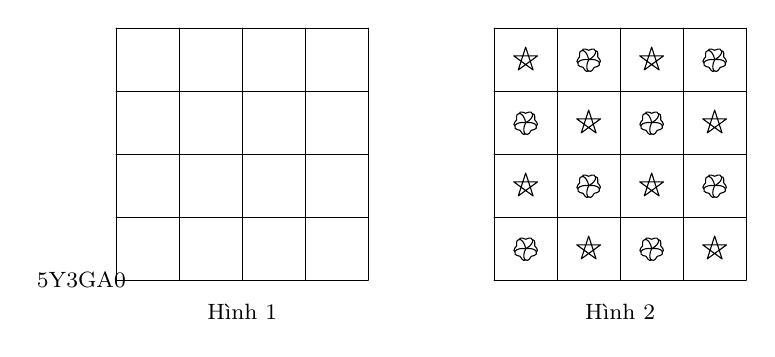
\begin{tikzpicture}[scale=0.8, font=\footnotesize, line join=round, line cap=round, >=stealth]
    %hidden: VM005
			\def\flower(#1,#2){
			\begin{scope}[shift={(#1,#2)}, scale=0.15]
				\foreach \a in {18,90,162,234,306}{
				\draw[rotate=\a, fill=white] (0,0) .. controls (0.5,1) and (1.5,1) .. (1,0) .. controls (1.5,-1) and (0.5,-1) .. (0,0);
				}
			\end{scope}
			}
			\def\starS(#1,#2){
			\begin{scope}[shift={(#1,#2)}, scale=0.2]
				\draw[fill=white] (90:1) -- (234:1) -- (18:1) -- (162:1) -- (306:1) -- cycle;
			\end{scope}
			}
			\begin{scope}
				\draw (0,0) grid (4,4);
				\node at (2,-0.5) {Hình 1};
			\end{scope}			
			\begin{scope}[xshift=6cm]
				\draw (0,0) grid (4,4);
				\starS(0.5,3.5); \flower(1.5,3.5); \starS(2.5,3.5); \flower(3.5,3.5);
				\flower(0.5,2.5); \starS(1.5,2.5); \flower(2.5,2.5); \starS(3.5,2.5);
				\starS(0.5,1.5); \flower(1.5,1.5); \starS(2.5,1.5); \flower(3.5,1.5);
				\flower(0.5,0.5); \starS(1.5,0.5); \flower(2.5,0.5); \starS(3.5,0.5);
				\node at (2,-0.5) {Hình 2};
			\end{scope}
    \node at (0,0){\href{5Y3GA0}{\tiny \phantom{5Y3GA0}}};
		\end{tikzpicture}
	\end{center}
	\par \shortans{$2\,502$}
	\loigiai{
		Gọi $A$ là tập hợp các cách trang trí mà mỗi hàng đều có đúng $2$ ngôi sao và $2$ bông hoa. \\
		Gọi $B$ là tập hợp các cách trang trí mà mỗi cột đều có đúng $2$ ngôi sao và $2$ bông hoa. \\
		Yêu cầu bài toán là tìm số cách trang trí thuộc tập hợp $A \cup B$. Ta có
		\[n(A\cup B) = n(A)+n(B)-n(A\cap B).\]
		\begin{itemize}
			\item Số phần tử của $A$ (mỗi hàng đều có đúng $2$ ngôi sao và $2$ bông hoa).\\
			Mỗi hàng có $4$ ô vuông, số cách chọn $2$ ô để dán ngôi sao là $C_4^2 = 6$ cách. \\
			Vì bảng có $4$ hàng động độc lập với nhau, nên số cách trang trí để mỗi hàng đều có $2$ ngôi sao là
			\[n(A) = 6 \cdot 6 \cdot 6 \cdot 6 = 6^4 = 1\,296 \text{ (cách).}\]
			\item Số phần tử của $B$ (mỗi cột đều có đúng $2$ ngôi sao và $2$ bông hoa).
			Tương tự như trường hợp hàng, số cách trang trí để mỗi cột đều có đúng $2$ ngôi sao là\\
			\[n(B) = 6^4 = 1\,296 \text{ (cách).}\]
			\item Số phần tử của  $A \cap B$ (cả cột và hàng đều có đúng $2$ ngôi sao và $2$ bông hoa). \\
			Đây là số cách xếp $2$ ngôi sao vào mỗi hàng và mỗi cột. Ta xét các trường hợp cho hàng thứ hai so với hàng thứ nhất ($6$ cách chọn hàng 1):
			\begin{enumerate}[\it TH1: ]
				\item Hàng 2 giống hệt hàng 1: Có $1$ cách chọn hàng 2. Khi đó hàng 3 và hàng 4 bắt buộc phải dán ngược lại với hàng 1. Có $6 \cdot 1 \cdot 1 = 6$ cách.
				\item Hàng 2 ngược hoàn toàn hàng 1: Có $1$ cách chọn hàng 2. Khi đó mỗi cột đã có $1$ sao. Hàng 3 có $\mathrm{C}_4^2=6$ cách chọn, hàng 4 là phần bù của hàng 3. Có $6 \cdot 1 \cdot 6 = 36$ cách.
				\item Hàng 2 có đúng $1$ vị trí sao trùng hàng 1: Có $\mathrm{C}_2^1 \cdot \mathrm{C}_2^1 = 4$ cách chọn hàng 2. Khi đó cặp hàng 3 và hàng 4 có đúng $2$ cách xếp để bổ sung đủ sao cho các cột. Có $6 \cdot 4 \cdot 2 = 48$ cách.
			\end{enumerate}
			Suy ra $n(A \cap B) = 6 + 36 + 48 = 90$ cách.
		\end{itemize}
		Số cách trang trí thỏa mãn mỗi hàng hoặc mỗi cột có $2$ sao là
		$$n(A\cup B) = n(A)+n(B)-n(A\cap B) = 1\,296 + 1\,296 - 90 = 2\,502 \text{ (cách).}$$
	}
\end{ex}

\begin{ex}%[Dự án 1O3C5B-VN-MT-15]%[2-KS-1-SoHaNoi-L1-2026,VM028]%[2D1V3-5]
	\immini[thm]{Cho hình vuông $ABCD$ có độ dài cạnh bằng $1$. Cung $AC$ là một phần tư đường tròn tâm $D$, bán kính $DA$ (tham khảo hình vẽ). Giả sử $P$ là điểm thay đổi trên cung $AC$ ($P$ khác $A$ và $C$). Tiếp tuyến tại điểm $P$ của cung $AC$ cắt các đoạn thẳng $AB$, $BC$ theo thứ tự tại các điểm $M$, $N$. Diện tích lớn nhất của tam giác $BMN$ bằng bao nhiêu (kết quả làm tròn đến hàng phần trăm)?
		}{
		\begin{tikzpicture}[scale=0.8,line cap=round,line join=round,font=\footnotesize,>=stealth]
    %hidden: VM005
			\def\a{4} \def\t{55}
			\path
				(0,0) coordinate (D)
				(\a,0) coordinate (C)
				(\a,\a) coordinate (B)
				(0,\a) coordinate (A)
				(\t:\a) coordinate (P)
				({\a*(1-sin(\t))/cos(\t)},\a) coordinate (M)
				(\a,{\a*(1-cos(\t))/sin(\t)}) coordinate (N);
			\draw (A)--(B)--(C)--(D)--cycle (C)arc(0:90:\a) (M)--(N);
			\fill[pattern=north east lines] (M)--(B)--(N)--cycle;
			\foreach \p/\ang in {D/225, C/-45, B/45, A/135, P/-2*\t, M/90, N/0} {
			\fill (\p) circle (1pt);
			\node at (\p) [shift={(\ang:8pt)}] {$\p$};
			}
    \node at (0,0){\href{1O3C5B}{\tiny \phantom{1O3C5B}}};
		\end{tikzpicture}
		}
		\par
		\shortans{$0{,}17$}
	\loigiai{
		\begin{center}
			\begin{tikzpicture}[scale=1,line cap=round,line join=round,font=\footnotesize,>=stealth]
    %hidden: VM005
				\def\a{4} \def\t{55}
				\path
					(0,0) coordinate (D)
					(\a,0) coordinate (C)
					(\a,\a) coordinate (B)
					(0,\a) coordinate (A)
					(\t:\a) coordinate (P)
					({\a*(1-sin(\t))/cos(\t)},\a) coordinate (M)
					(\a,{\a*(1-cos(\t))/sin(\t)}) coordinate (N);		
				\draw [->](D)--($(C)+(1,0)$) node [below]{$x$};
				\draw [->](D)--($(A)+(0,1)$) node [left]{$y$};
				\draw (A)--(B)--(C)--(D)--cycle (C)arc(0:90:\a) (M)--(N);
				\fill[pattern=north east lines] (M)--(B)--(N)--cycle;
				\foreach \p/\ang in {D/225, C/-45, B/45, A/135, P/-2*\t, M/90, N/0} {
				\fill (\p) circle (1pt);
				\node at (\p) [shift={(\ang:8pt)}] {$\p$};
			}
				%		\fill (D) circle (1pt) node [shift={(-135:0.3)}]{$O$};
    \node at (0,0){\href{1O3C5B}{\tiny \phantom{1O3C5B}}};
			\end{tikzpicture}
		\end{center}
		{\it Cách 1:}
		Chọn hệ trục tọa độ $Oxy$ sao cho $O\equiv D(0;0)$, $C(1;0)$, $A(0;1)$. Khi đó $B(1;1)$.\\
		Do cung $AC$ thuộc đường tròn tâm $D(0;0)$ bán kính $r=1$ nên thỏa mãn phương trình $x^2+y^2=1$. \\
		Vì $P(x_0,y_0)$ thuộc cung $AC$ nên $x_0^2+y_0^2=1$ với $0<x_0<1$, $0<y_0<1$.\\
		Tiếp tuyến tại $P(x_0,y_0)$ của đường tròn $x^2+y^2=1$ có phương trình là $x_0x+y_0y=1$.
		\begin{itemize}
			\item Đường thẳng $AB$ có phương trình $y=1$, tọa độ điểm $M$ thỏa mãn
			\[\heva{&x_0x+y_0y=1\\&y=1}\Leftrightarrow \heva{&x=\dfrac{1-y_0}{x_0}\\&y=1.}
			\]
			Suy ra $M\left(\dfrac{1-y_0}{x_0};1\right) \Rightarrow BM=1-\dfrac{1-y_0}{x_0}=\dfrac{x_0+y_0-1}{x_0}$.
			\item Đường thẳng $CB$ có phương trình $x=1$, tọa độ điểm $N$ thỏa mãn
			\[\heva{&x_0x+y_0y=1\\&x=1}\Leftrightarrow \heva{&x=1\\&y=\dfrac{1-x_0}{y_0}.}
			\]
			Suy ra $N\left(1;\dfrac{1-x_0}{y_0}\right) \Rightarrow BN=1-\dfrac{1-x_0}{y_0}=\dfrac{x_0+y_0-1}{y_0}$.
		\end{itemize}
		Xét $\triangle BMN$ vuông tại $B$,
		\[
		S_{BMN}=\dfrac{1}{2} BM\cdot BN=\dfrac{1}{2}\cdot\dfrac{(x_0+y_0-1)^2}{x_0y_0}.
		\]
		Ta có $x_0y_0=\dfrac{\left(x_0+y_0\right)^2-\left(x_0^2+y_0^2\right)}{2}=\dfrac{\left(x_0+y_0\right)^2-1}{2}$ (vì $x_0^2+y_0^2=1$).\\
		Từ đây suy ra $\left(x_0+y_0\right)^2>1\Rightarrow x_0+y_0>1$.\\
		Đặt $t=x_0+y_0$, ta có
		$	S=\dfrac{1}{2}\cdot\dfrac{(t-1)^2}{\dfrac{t^2-1}{2}}=\dfrac{(t-1)^2}{t^2-1}=\dfrac{t-1}{t+1}$ với $t>1$.\\
		Lại có $\left(x_0+y_0\right)^2\leq 2\left(x_0^2+y_0^2\right)=2\cdot 1=2\Rightarrow x_0+y_0 \leq \sqrt{2}\Rightarrow t\leq \sqrt{2}$ (vì $x_0+y_0>1$).\\
		Xét hàm số $f(t)=\dfrac{t-1}{t+1}$ với $1<t\le\sqrt2$.\\
		Ta có $f'(t)=\dfrac{2}{(t+1)^2}$; $f'(t)>0$,\,$\forall x\in \left(1;\sqrt2\right)$.\\
		Suy ra $f(t)$ đồng biến trên $\left(1;\sqrt2\right]\Rightarrow f(t)\leq f\left(\sqrt2\right)$.\\
		Dấu \lq\lq=\rq\rq\ xảy ra khi và chỉ khi $t= \sqrt2$, lúc đó $x_0=y_0=\dfrac{1}{\sqrt{2}}$.\\
		Vì $f\left(\sqrt2\right)=\dfrac{\sqrt2-1}{\sqrt2+1}=3-2\sqrt2\approx0{,}17$	nên giá trị lớn nhất của hàm số $f(t)$ (cũng là giá trị lớn nhất của $S_{BMN}$) là $3-2\sqrt2\approx0{,}17$.\\
		Vậy diện tích lớn nhất của tam giác $BMN$ (làm tròn đến hàng phần trăm) là $0{,}17$.\\
		{\it Cách 2:}
		Đặt $BM=x$, $BN=y$, điều kiện $0<x<1$ và $0<y<1$.\\
		Ta có $MA=1-x$ và $NC=1-y$. \\
		Theo tính chất về hai tiếp tuyến xuất phát từ một điểm của đường tròn suy ra $MP=1-x$, $NP=1-y$.\\
		Ngoài ra, $MN=MP+PN=1-x+1-y=2-x-y$.\\
		Xét tam giác vuông $BMN$ có
		\begin{eqnarray*}
			&&BM^2+BN^2=MN^2\\
			&\Leftrightarrow& x^2+y^2=(2-x-y)^2\\
			&\Leftrightarrow&x^2+y^2 = 4-4(x+y)+(x+y)^2\\
			&\Leftrightarrow& 4-4x-4y+2xy=0\\
			&\Leftrightarrow& xy+2=2(x+y).\qquad (1)
		\end{eqnarray*}
		Mặt khác, $(1)\Leftrightarrow(2-x)(2-y) = 2$.\\
		Vì $0<x<1$, $0<y<1$ nên $2>2-x>1$, $2>2-y>1$ và $4-x-y>2$. \\
		Ta có
		\begin{eqnarray*}
			&&\dfrac{(2-x+2-y)^2}{4}\geq (2-x)(2-y)\\
			&\Leftrightarrow &\dfrac{(4-x-y)^2}{4}\geq 2\\
			&\Leftrightarrow &(4-x-y)^2\geq 8\\
			&\Leftrightarrow &4-x-y\geq 2\sqrt{2}\\
			&\Leftrightarrow &x+y\leq 4-2\sqrt{2}.\qquad (2)
		\end{eqnarray*}
		Mặt khác $\triangle BMN$ vuông tại $B$ nên $S_{BMN}=\dfrac{1}{2} BM\cdot BN=\dfrac{1}{2}xy$.\hfill $(3)$\\
		Từ $(1)$ và $(3)$, kết hợp với $(2)$ suy ra
		\[S_{BMN}=\dfrac{1}{2}(2x+2y-2)=x+y-1\leq3-2\sqrt{2}.
		\]
		Dấu \lq\lq=\rq\rq\ xảy ra khi và chỉ khi
		\[\heva{&2-x = 2-y\\&xy+2=2(x+y)}\Leftrightarrow\heva{&x =y\\&x^2-4x+2=0}\Leftrightarrow x =y=2-\sqrt{2}.
		\]
		Ta có $3-2\sqrt{2}\approx 0{,}17$ (làm tròn đến hàng phần trăm).\\
		Vậy diện tích lớn nhất của tam giác $BMN$ là $0{,}17$.\\
	}
\end{ex}

\begin{ex}%[Dự án 1KCG6H-VN-MT-15]%[2-KS-1-SoHaNoi-L1-2026,VM028]%[1H8H6-2]
	\immini[thm]{Cho hình chóp tứ giác $S.ABCD$ có đáy $ABCD$ là hình vuông cạnh bằng $2$. Biết rằng $SA$ vuông góc với mặt phẳng $(ABCD)$ và $SA = \sqrt{6}$ (tham khảo hình vẽ). Góc phẳng nhị diện $[S, BD,C]$ có số đo bằng bao nhiêu độ?
		}{
		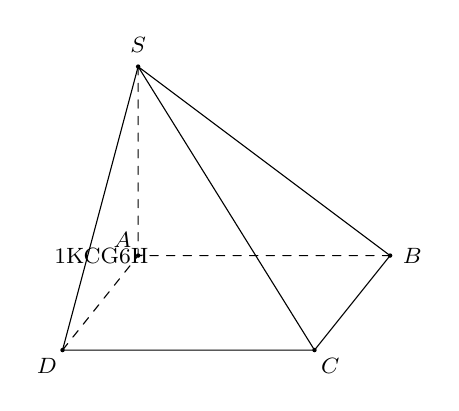
\begin{tikzpicture}[scale=0.8,line cap=round,line join=round,font=\footnotesize,>=stealth]
    %hidden: VM005
			\def\h{3} \def\w{4}
			\path
				coordinate (S) at (0,\h)
				coordinate (A) at (0,0)
				coordinate (B) at (\w,0)
				coordinate (D) at (-1.2,-1.5)
				coordinate (C) at (\w-1.2,-1.5);
			\draw[dashed] (S)--(A) (D)--(A)--(B);
			\draw (S)--(D)--(C)--(B)--(S)--(C);
			\foreach \p/\a in {S/90, A/135, B/0, C/-45, D/225}
			\fill (\p) circle (1pt) node [shift={(\a:8pt)}] {$\p$};
    \node at (0,0){\href{1KCG6H}{\tiny \phantom{1KCG6H}}};
		\end{tikzpicture}
		}
		\par
		\shortans{$120$}
	\loigiai{
		\begin{center}
			\begin{tikzpicture}[scale=1,line cap=round,line join=round,font=\footnotesize,>=stealth]
    %hidden: VM005
				\def\h{3} \def\w{4}
				\path
					coordinate (S) at (0,\h)
					coordinate (A) at (0,0)
					coordinate (B) at (\w,0)
					coordinate (D) at (-1.2,-1.5)
					coordinate (C) at (\w-1.2,-1.5)
					coordinate (O) at ($(A)!0.5!(C)$);
				\draw[dashed] (S)--(A)--(C) (O)--(S) (D)--(A)--(B)--cycle;
				\draw (S)--(D)--(C)--(B)--(S)--(C);
				\foreach \p/\a in {S/90, A/135, B/0, C/-45, D/225,O/-90}
				\fill (\p) circle (1pt) node [shift={(\a:8pt)}] {$\p$};
				\draw pic [draw, angle radius=0.3cm,angle eccentricity=1.7] {angle = C--O--S};
    \node at (0,0){\href{1KCG6H}{\tiny \phantom{1KCG6H}}};
			\end{tikzpicture}
		\end{center}
		Gọi $O=AC\cap BD$ suy ra $O$ là trung điểm của $AC$ và $BD$. Ta có
		\[\heva{&AC\perp BD\\&SA\perp(ABCD)\Rightarrow SA\perp BD}\Rightarrow (SAC)\perp BD.
		\]
		Cắt nhị diện $[S,BD,C]$ có cạnh $BD$ bởi mặt phẳng $(SAC)$ ta được góc phẳng nhị diện $\widehat{SOC}$.\\
		Vì $ABCD$ là hình vuông cạnh bằng $2$ nên $AC=2\sqrt2$, $AO=OC=\sqrt2$.\\
		Ta có
		\[SO=\sqrt{SA^2+AO^2}=\sqrt{6+2}=2\sqrt2;\quad SC=\sqrt{SA^2+AC^2}=\sqrt{6+8}=\sqrt{14}.
		\]
		Áp dụng định lý côsin trong $\triangle SOC$ ta được
		\[
		\cos\widehat{SOC}=\dfrac{SO^2+OC^2-SC^2}{2SO\cdot OC}
		=\dfrac{8+2-14}{2\cdot 2\sqrt2\cdot\sqrt2}=-\dfrac{1}{2}\Rightarrow \widehat{SOC}=120^\circ.
		\]
		Vậy góc phẳng nhị diện $[S,BD,C]$ bằng $120^\circ$.
	}
\end{ex}

\begin{ex}%[Dự án 3D36QL-VN-MT-15]%[2-KS-1-SoHaNoi-L1-2026,VM028]%[2D4C3-2]
	\immini[thm]{Trong lưới ô vuông có hai đường parabol như hình vẽ. Biết rằng mỗi ô vuông nhỏ có cạnh bằng $1$\,cm. Diện tích của hình phẳng trong lưới ô vuông được giới hạn bởi hai đường parabol (phần gạch chéo) bằng bao nhiêu centimet vuông (kết quả làm tròn đến hàng phần trăm)?
		}{
		\begin{tikzpicture}[scale=0.8,line cap=round,line join=round,font=\footnotesize,>=stealth,x=0.7cm, y=0.7cm]
    %hidden: VM005
			\def\mydomain{-4:4}
			\draw[step=1,dashed,gray!60] (-4,0) grid (4,8);
			\draw (-4,0) rectangle (4,8);
			\fill[pattern=north east lines] plot[domain=\mydomain](\x,{(11/48)*(\x)^2-(1/8)*\x+11/6})--plot[domain=4:-4](\x,{0.5*(\x)^2})--cycle;
			\draw plot[domain=\mydomain] (\x,{(11/48)*(\x)^2-(1/8)*\x+11/6}) plot[domain=\mydomain] (\x,{0.5*(\x)^2});
			\fill (-4,8) circle (1pt) (4,8) circle (1pt) (0,0) circle (1pt) (-4,6) circle (1pt) (-2,3) circle (1pt) (4,5) circle (1pt) ;
			\draw[dashed] (-4,3)-|(-2,0);
    \node at (0,0){\href{3D36QL}{\tiny \phantom{3D36QL}}};
		\end{tikzpicture}
		}
		\par
		\shortans{$9{,}76$}
	\loigiai{
		Chọn hệ trục tọa độ $Oxy$ có gốc $O(0;0)$ tại trung điểm cạnh dưới của lưới ô vuông $8 \times 8$, trục hoành và trục tung như hình vẽ. Đơn vị mỗi ô vuông nhỏ tương ứng với $1$\,cm.
		\begin{center}
			\begin{tikzpicture}[scale=0.8,line cap=round,line join=round,font=\footnotesize,>=stealth,dot/.style={circle, fill=red, inner sep=1.2pt}]
    %hidden: VM005
				\def\mydomain{-4:4}
				\draw[step=1,dashed,gray!60] (-4,0) grid (4,8);
				\draw (-4,0) rectangle (4,8);
				\fill[pattern=north east lines] plot[domain=\mydomain](\x,{(11/48)*(\x)^2-(1/8)*\x+11/6})--plot[domain=4:-4](\x,{0.5*(\x)^2})--cycle;
				\draw plot[domain=\mydomain] (\x,{(11/48)*(\x)^2-(1/8)*\x+11/6})
					node [xshift=-14pt,yshift=-40pt]{$(P_2)$};
				\draw plot[domain=\mydomain] (\x,{0.5*(\x)^2})
					node [xshift=-14pt,yshift=-12pt]{$(P_1)$};
				\draw[dashed] (0,3)-|(-2,0);
				\draw[->] (-5,0)--(5,0)node[below]{$x$};
				\draw[->] (0,-1)--(0,9)node[left]{$y$};
				\path
					coordinate (A) at (-4,8)
					coordinate (B) at (-4,6)
					coordinate (C) at (4,8)
					coordinate (D) at (4,5)
					coordinate (E) at (-2,3)
					coordinate (O) at (0,0)	;
				\foreach \d/\n in {A/135,B/180,C/45,D/0,E/45,O/-135}
				\fill (\d) circle (1pt) node [shift={(\n:0.3cm)}] {$\d$};
				\foreach \x/\y/\t/\p in {-4/0/-90/-4,-2/0/-90/-2,4/0/-90/4,0/3/135/3,0/8/135/8,0/5/135/5,0/6/135/6}
				\fill (\x,\y) circle (1pt) node [shift={(\t:0.3cm)}] {$\p$};
    \node at (0,0){\href{3D36QL}{\tiny \phantom{3D36QL}}};
			\end{tikzpicture}
		\end{center}
		Khi đó
		\begin{itemize}
			\item Parabol $(P_1)$ đi qua các điểm $O(0;0)$, $A(-4;8)$, $C(4;8)$. \\
			Gọi $(P_1)\colon y=ax^2+bx+c$, ta có hệ phương trình
			\[\heva{&c=0\\&16a-4b+c=8\\&16a+4b+c=8}\Leftrightarrow \heva{&c=0\\&b=0\\&a=\dfrac{1}{2}}\Rightarrow (P_1)\colon y= \dfrac{1}{2}x^2.
			\]
			\item Parabol $(P_2)$ đi qua các điểm $B(-4;6)$, $D(4;5)$, $E(-2;3)$. \\
			Gọi $(P_2)\colon y=a'x^2+b'x+c'$, ta có hệ phương trình
			\[\heva{&16a'-4b'+c'=6\\&16a'+4b'+c'=5\\&4a'-2b'+c'=3}\Leftrightarrow \heva{&a'=\dfrac{11}{48}\\&b'=-\dfrac{1}{8}\\&c'=\dfrac{11}{6}}\Rightarrow (P_2)\colon y = \dfrac{11}{48}x^2-\dfrac{1}{8}x+\dfrac{11}{6}.
			\]
		\end{itemize}
		Phương trình hoành độ giao điểm của hai parabol là
		\allowdisplaybreaks
		\begin{eqnarray*}
			&&\dfrac{1}{2}x^2=\dfrac{11}{48}x^2-\dfrac{1}{8}x+\dfrac{11}{6}\\
			&\Leftrightarrow&\dfrac{13}{48}x^2+\dfrac{1}{8}x-\dfrac{11}{6} = 0\\
			&\Leftrightarrow&13x^2+6x-88 = 0\\
			&\Leftrightarrow&\hoac{
			&x = \dfrac{-3+\sqrt{1\,153}}{13}\\
			&x = \dfrac{-3-\sqrt{1\,153}}{13}.}
		\end{eqnarray*}
		Hình phẳng được giới hạn bởi hai parabol trên đoạn $[-4; 4]$ có diện tích là
		\begin{align*}
			S &= \displaystyle\int\limits_{-4}^{4} \left|\dfrac{1}{2}x^2-\bigg(\dfrac{11}{48}x^2-\dfrac{1}{8}x+\dfrac{11}{6}\bigg)\right| \mathrm{d}x\\
			&= \displaystyle\int\limits_{-4}^{4} \left|\dfrac{13}{48}x^2+\dfrac{1}{8}x-\dfrac{11}{6}\right| \mathrm{d}x\\
			&= \displaystyle\int\limits_{-4}^{x_1} \big|h(x)\big| \mathrm{\,d}x+\displaystyle\int\limits_{x_1}^{x_2} \big|h(x)\big| \mathrm{\,d}x+\displaystyle\int\limits_{x_2}^{4} \big|h(x)\big| \mathrm{\,d}x\\
			&= \displaystyle\int\limits_{-4}^{x_1} h(x) \mathrm{\,d}x+\displaystyle\int\limits_{x_1}^{x_2} \big(-h(x)\big) \mathrm{\,d}x+\displaystyle\int\limits_{x_2}^{4} h(x) \mathrm{\,d}x\text{,}
		\end{align*}
		trong đó $x_1=\dfrac{-3-\sqrt{1\,153}}{13}$, $x_2=\dfrac{-3+\sqrt{1\,153}}{13}$ và $h(x) = \dfrac{13}{48}x^2+\dfrac{1}{8}x-\dfrac{11}{6}$.\\
		Ta có $h(x) =\dfrac{13}{48}x^2+\dfrac{1}{8}x-\dfrac{11}{6}$ có một nguyên hàm là $F(x) = \dfrac{13}{144}x^3+\dfrac{1}{16}x^2-\dfrac{11}{6}x$.\\
		Khi đó
		\[S = \big(F(x_1)-F(-4)\big)-\big(F(x_2)-F(x_1)\big)+\big(F(4)-F(x_2)\big)\approx9{,}7554.
		\]
		Làm tròn đến hàng phần trăm, ta được kết quả là $9{,}76$\,cm$^2$.
	}
\end{ex}

\Closesolutionfile{ans}
\Closesolutionfile{ansbook}
\begin{indapan}
	{ans/ans\currfilebase}
\end{indapan}